\documentclass{article}

\usepackage{graphicx}

\renewcommand{\labelenumii}{\theenumii}
\renewcommand{\theenumii}{\theenumi.\arabic{enumii}.}
\renewcommand{\theenumiii}{\theenumii\arabic{enumiii}.}


\begin{document}
\begin{figure}[t!]
	
\includegraphics[width= \linewidth]{PolimiLogo.png}
	\begin{center}
	Politecnico di Milano\\[4pt]
	AA 2018-2019  \\[4pt]
	Computer Science and Engineering \\[4pt]
	\begin{large}
	Software Engineering 2 Project
	\end{large}
	\end{center}
\end{figure}
\begin{flushright}
\begin{large}
Dalle Rive Fabio - 920082 \\[4pt]
Di Giacomantonio Marco - 846515 \\[4pt]
\end{large}
\end{flushright}
\newpage
{\Large\textbf{Table of Contents}}
	\begin{enumerate}
			\item Introduction
			\begin{enumerate}
				\item Purpose
				\item Scope
				\item Definitions, Acronyms, Abbreviations
				\begin{enumerate}
					\item Definitions
					\item Acronyms
					\item Abbreviations
				\end{enumerate}
				\item Document structure
			\end{enumerate}
			\item Architectural Design
			\begin{enumerate}
				\item Overview
				\item High Level Architecture
				\item Component View
				\item Deployment View
				\item Runtime View
				\item Component Interfaces
				\item Selected architectural styles and patterns
				\begin{enumerate}
				\item Overall Architecture
				\item Design Pattern
				\end{enumerate}
				\item Other Design Decisions
			\end{enumerate}
			\item User Interfaces Design
			\item Requirements Traceability
			\item Implementation, Integration and Test Plan
			\item Effort Spent
			\item Resources
	\end{enumerate}
	\newpage
\section{Introduction}
\subsection{Purpose}
The purpose of this document is to give more technical details than the RASD about TrackMe system.
It provides an overall guidance to the architecture of the software product and therefore it is primarily addressed to the software development.
\subsection{Scope}
The project Data4Help aims to build a system that allows third parties to monitor the position and health status of users. All the data are collected by TrackMe, the company that wants to develop Data4Help, and are shared with other companies which are interested in those data. Furthermore, TrackMe wants to develop AutomatedSOS, a system build on top of Data4Help, designed for elderly people. It is able to intervene by calling an ambulance if the health parameters of the user are below some fixed thresholds.
The main target group of the application are the companies interested in users' data.
After registration, these companies can request:
\begin{itemize}
\item Access to the data of some specific user.
\item Access to anonymized data of groups of users.
\end{itemize}
Another terget group are elderly people, to whom is addessed AutomatedSOS, a non-intrusive SOS service. It is build on top of Data4Help. This service is designed to monitor health status of users and to send an ambulance to the location of the user if some parameters are below some specified thresholds.
\subsection{Definitions, Acronyms, Abbreviations}
\subsubsection{Acronyms}
\begin{itemize}
\item API: Application Programming Interface
\item DB: Database
\item DBMS: Database Management System 
\item DD: Design Document
\item GPS: Global Positioning System
\item GUI: Graphical User Interface
\item MVC: Model View Controller
\item RASD: Requirements Analysis and Specifications Document
\item UI: User Interface
\item SSN: Social Security Number
\end{itemize}
\subsubsection{Abbreviations}
\begin{itemize}
\item {[Gn]: n-th goal}
\item {[Rn]: n-th functional requirement}
\end{itemize}
\subsection{Document structure}
\begin{itemize}
 \item Introduction: this section introduces the design document. It explains the utility of the project, text conventions and the framework of the document.
\item Architecture Design: this section illustrates the main components of the system and the relationships between them, providing information about their operating principles and deployment. This section will also focus on the main architectural styles and patterns adopted in the design of the system.\newline
This section is divided into different parts:\newline
\textit{1. Overview}: this sections explains the tiers division of our application;\newline
\textit{2. High level architecture}: this sections gives a high-level view of the components of the application and how they communicate;\newline
\textit{3. Component view}: this sections gives a more detailed view of the components of the applications;\newline
\textit{4. Deploying view}: this section shows the components that must be deployed;\newline
\textit{5. Runtime view}: sequence diagrams are represented in this section to show how our application deals with different tasks;\newline
\textit{6. Component interfaces}: the interfaces between the components are presented in this section;\newline
\textit{7. Selected architectural styles and patterns}: this section explains the architectural choices taken during the creation of the application and the design pattern used;\newline
\textit{8. Other design decisions}.
\item User Interface Design: this section presents mockups about the User Interface.
\item Requirements Traceability: this section aims to explain how the decisions taken in the RASD are linked to design elements.
\item Implementation, Integration and test plan: identifies the order in which it is planned to implement the subcomponents of the system and the order in which it is planned to integrate such subcomponents and test the integration.
\end{itemize}
\newpage
\section{Architectural Design}
\subsection{Overview}
The application uses a three layers architecture.
\begin{itemize}
\item \textbf{Presentation tier}: This layer is used only by companies that want to access to users' data. The user interface consists of a website accessible from a browser. Each web page contains some JavaScript element in order to enable client-side interaction;
\item \textbf{Tier One}: This layer is only used from the background app running on the smart watch. The function of this layer is to communicate with the server all the data gathered form the sensor present on the smart watch. Data are then communicated to the AppServer every 30 seconds. Since this is the first time we present this concept of data transferring in the project let's look at it in more detail. The system-to-be need to operate as a collector of data gathered by the smart watch. Since it is not feasible that a server asks each smart watch to communicate the data, we need a software module, in the client side, that every \emph{tot} seconds ( here 30s ) sends data to the AppServer. This module is developed in Tier One. In the rest of the project we will not develop the client side of the application, and we will focus on the server side, nevertheless the presence of this module must be kept in mind.   
\item \textbf{Business Logic tier}: This second layer interacts with the Presentation tier and with Tier One. As regards the interaction with the Presentation tier it enables all the functionality listed in the RASD document, while the interaction with Tier One consists of the processing of the data coming from the user. This layer also communicates with the database in order to permanently store data and with the external services.
\item \textbf{Persistence tier}: This layer purpose is to save all the users' (e.g. current position, heartbeat...) and companies' (single user and group user request) data. It shows some interfaces that enable communication with the business logic tier, letting the second level access data.
\end{itemize}
\begin{figure}[h!]
\centering
	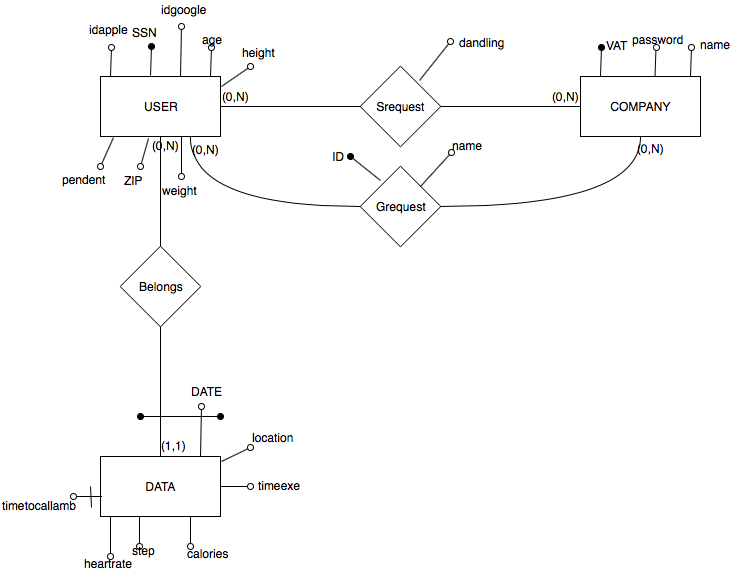
\includegraphics[width= 80mm, scale=0.7]{ER.png}
\end{figure}
Here is presented a possible entity-relationship model for the persistence tier.
\begin{figure}	
	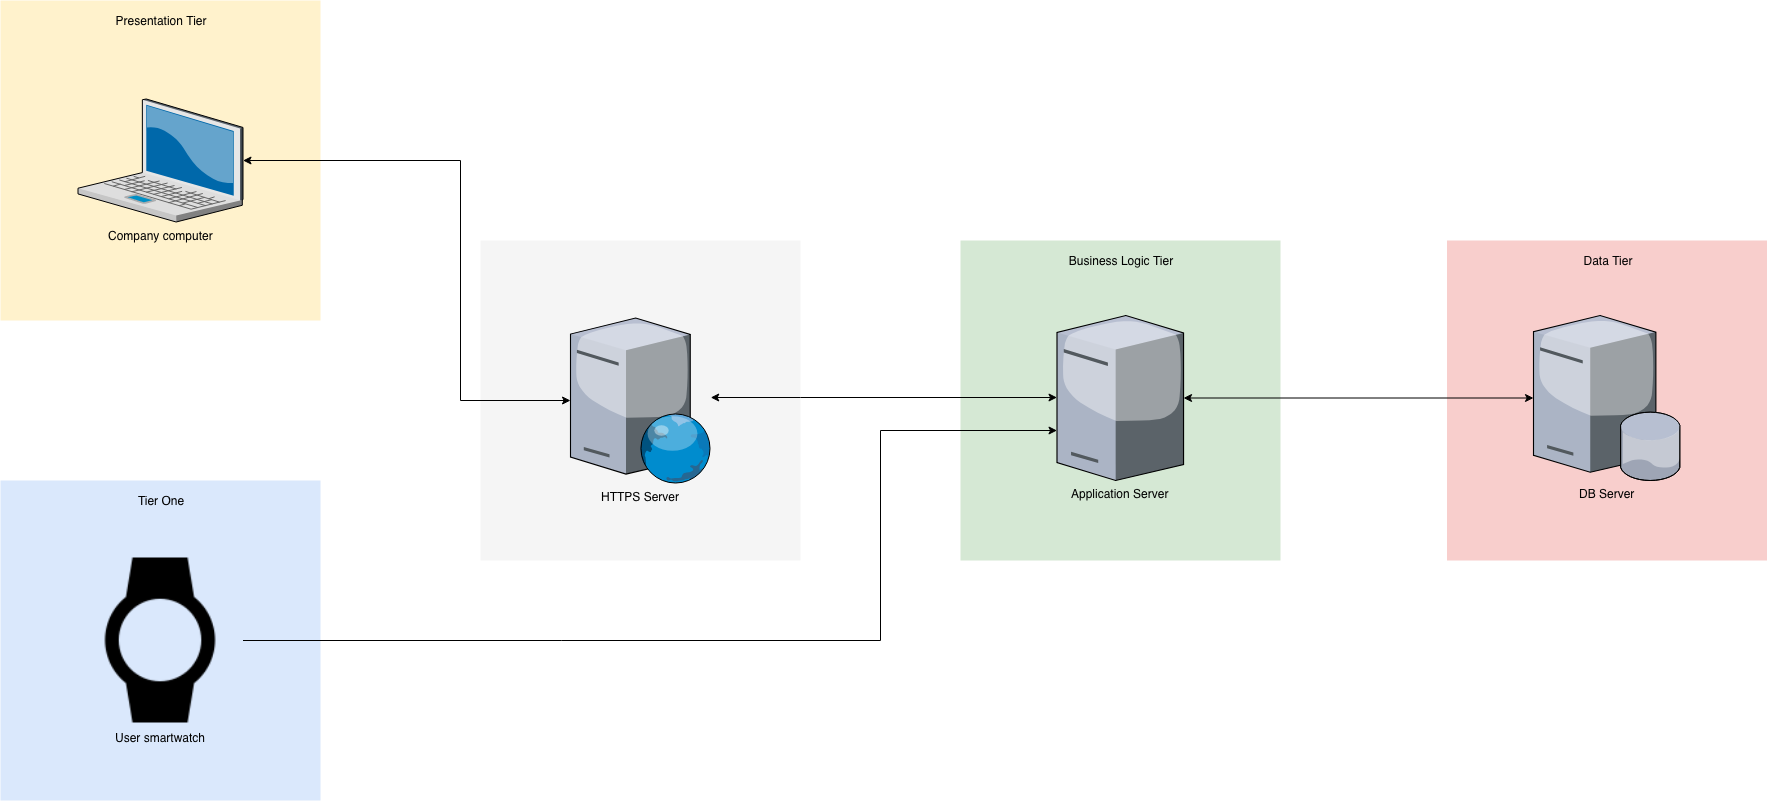
\includegraphics[width= \linewidth]{tier.png}
\end{figure}
\newpage
\newpage
\subsection{High Level Architecture}
\begin{figure}[h!]
\centering
    \textbf{}\par\medskip
	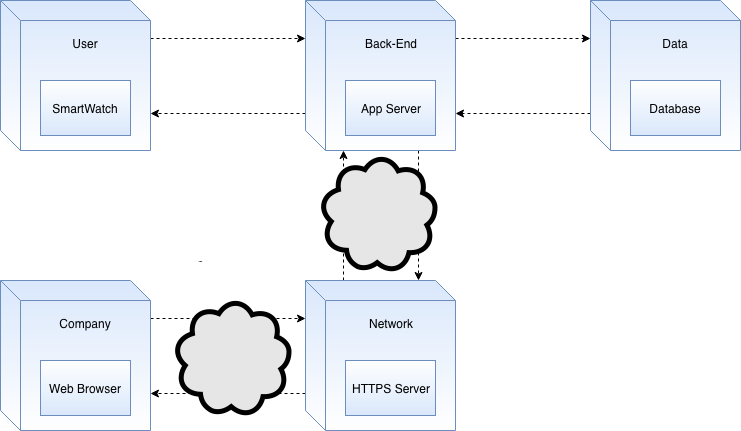
\includegraphics[width= \linewidth]{highlevel.png}
\end{figure}
The figure above describes the high-level architecture of the system. All the actors are represented and how they interact with each other.
Each tier is mapped with a high level architecture block, as represented in the table above.
\begin{table}[]
\begin{tabular}{|c|c|c|c|c|}
\hline
 & \begin{tabular}[c]{@{}c@{}}User\\ smart watch\end{tabular} & \begin{tabular}[c]{@{}c@{}}Company\\ Web Browser\end{tabular} & \begin{tabular}[c]{@{}c@{}}BackEnd\\ App Server\end{tabular} & \begin{tabular}[c]{@{}c@{}}Data\\ Database\end{tabular} \\ \hline
Presentation Tier &  & X &  &  \\ \hline
Tier One & X &  &  &  \\ \hline
Business Logic Tier &  &  & X &  \\ \hline
Persistence tier &  &  &  & X \\ \hline
\end{tabular}
\end{table}
\newpage
\subsection{Component View}
\begin{figure}[h!]
\centering
    \textbf{}\par\medskip
	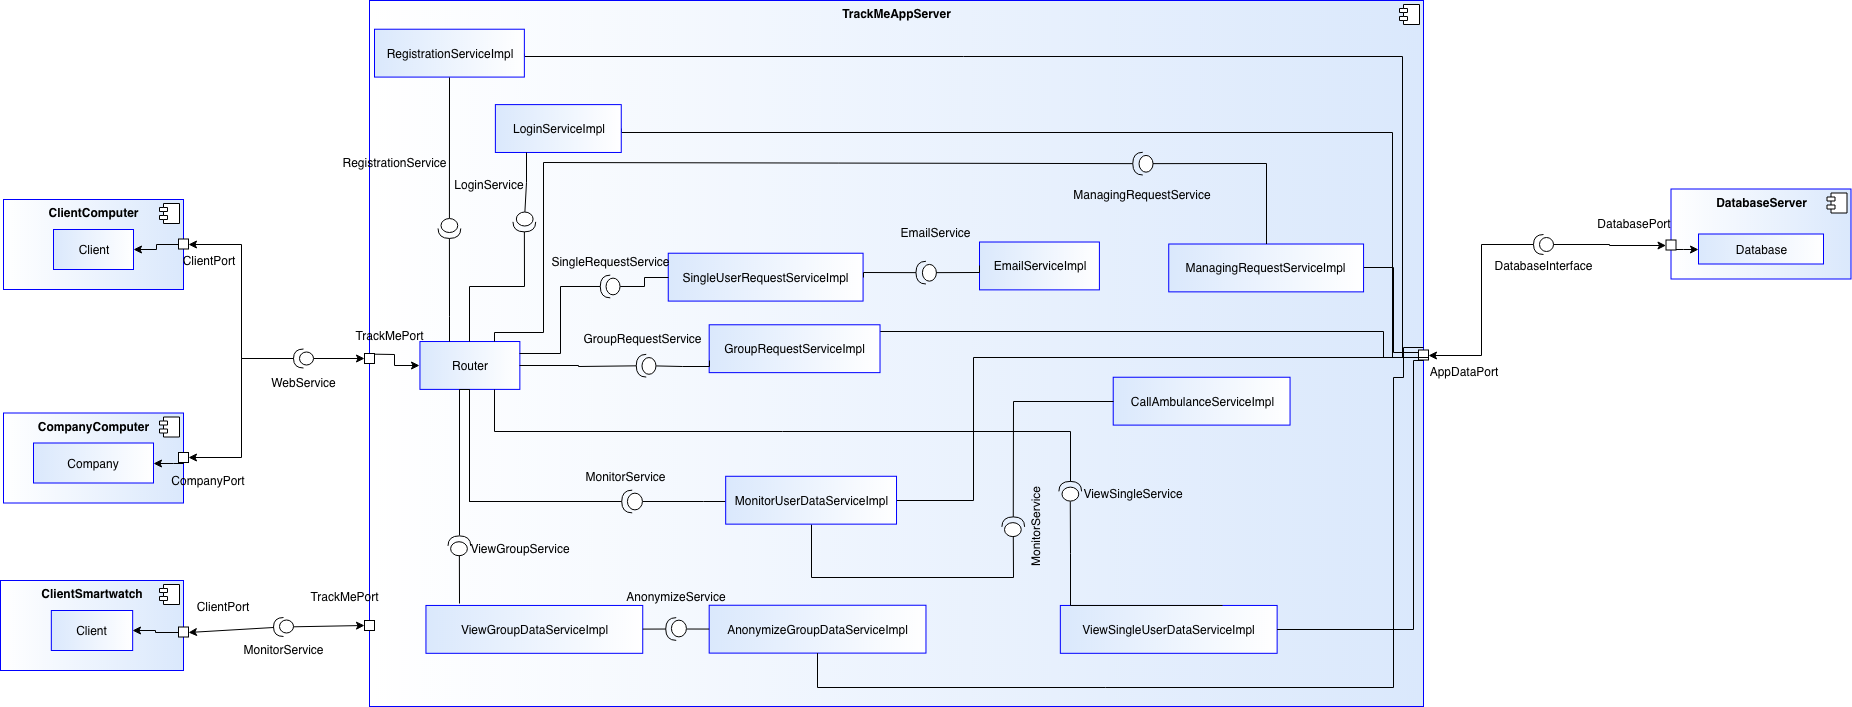
\includegraphics[width= \linewidth]{comp.png}
\end{figure}
This diagram shows the components and how they interact with each other. All of them are part of the system, apart from the email service that is external. The email service is only used to send emails between the company and the user and viceversa. \newline
The main component is the application server and it consists of the following parts:
\begin{itemize}
\item LoginService: responsible for authentication of the companies;
\item Registration Service: responsible for registration of companies and of single users by using their Apple or Google credentials;
\item Single User Request Service: enables companies to formulate a request based on the user SSN in order to access data of a single user;
\item GroupRequestService: enables companies to formulate a request in order to access data of a group of users with some specific traits. Furthermore it is responsible for showing an answer to the company request, positive or negative;
\item EmailService: external service used to forward companies request to single users and to let them answer these requests;
\item ManagingRequestService: enables single user to accept or decline a request by clicking on the corresponding link received in the single user request email that redirects him to our website;
\item CallAmbulanceService: external service responsible for calling an ambulance if users heart rate is below \emph{Threshold}. With the term \emph{calling an ambulance} we indicate all the process that this module must follow in order to contact the ambulance and share the user's current location. Due to the fact that this is an external service, that is offered to the system-to-be, the only things that can be said at this point is that during the development of this module, programmers will be provided with all the materials needed to communicate with this module(i.e \emph{primitive calls,...});
\item ViewSingleUserDataService: shows data of a single user to a company. This module query the DB and create a user-friendly graphical representation of data obtained by DB;
\item AnonymizeGroupDataService: responsible for anonymizing data of a group of users. This is the component that will actually carry out the process of building a possible group, based on the filter present in the GroupUserRequest issued by a company. All this process is based on the possibility to query the DB and build the group after having verify that more than 1000 user are part of it. This module must also be able to build a sort of intermediate representation of the data, which is sent to the ViewGroupDataServiceImpl, starting from the result of the queries;
\item ViewGroupDataService: shows data of a group of users to a company. This module will get the data to display directly from AnonymizeData;
\item MonitorUserDataService: responsible for receiving data from the client every 30 seconds. If the user is subscribed to AutomatedSOS checks if the data are below a certain value and communicates with Call Ambulance Service. Here it is not meant to go deeper in the development process, but due to the distributed nature of this application we suggest to use message queues to handle the incoming data;
\item Router: dispatch a request to the relevant service component;
\end{itemize}
The following diagram shows the Model of the System-to-be. 
\begin{figure}[h!]
\centering
    \textbf{}\par\medskip
	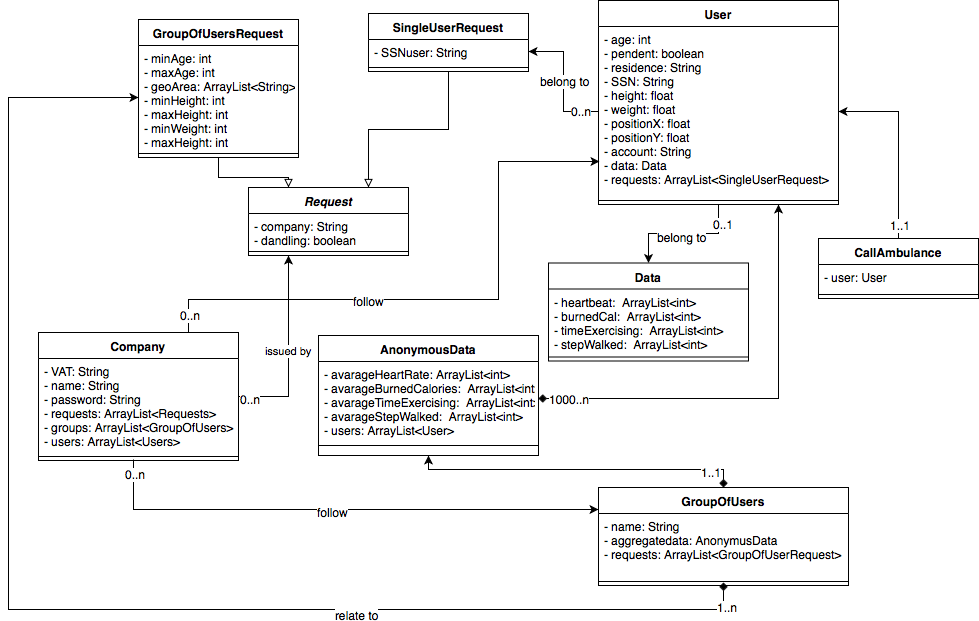
\includegraphics[width= \linewidth]{model.png}
\end{figure}
\newpage
The following diagram represents the UML of the whole system with emphasis on the View component and is shown the interaction between the result and the model.
\begin{figure}[h!]
\centering
    \textbf{}\par\medskip
	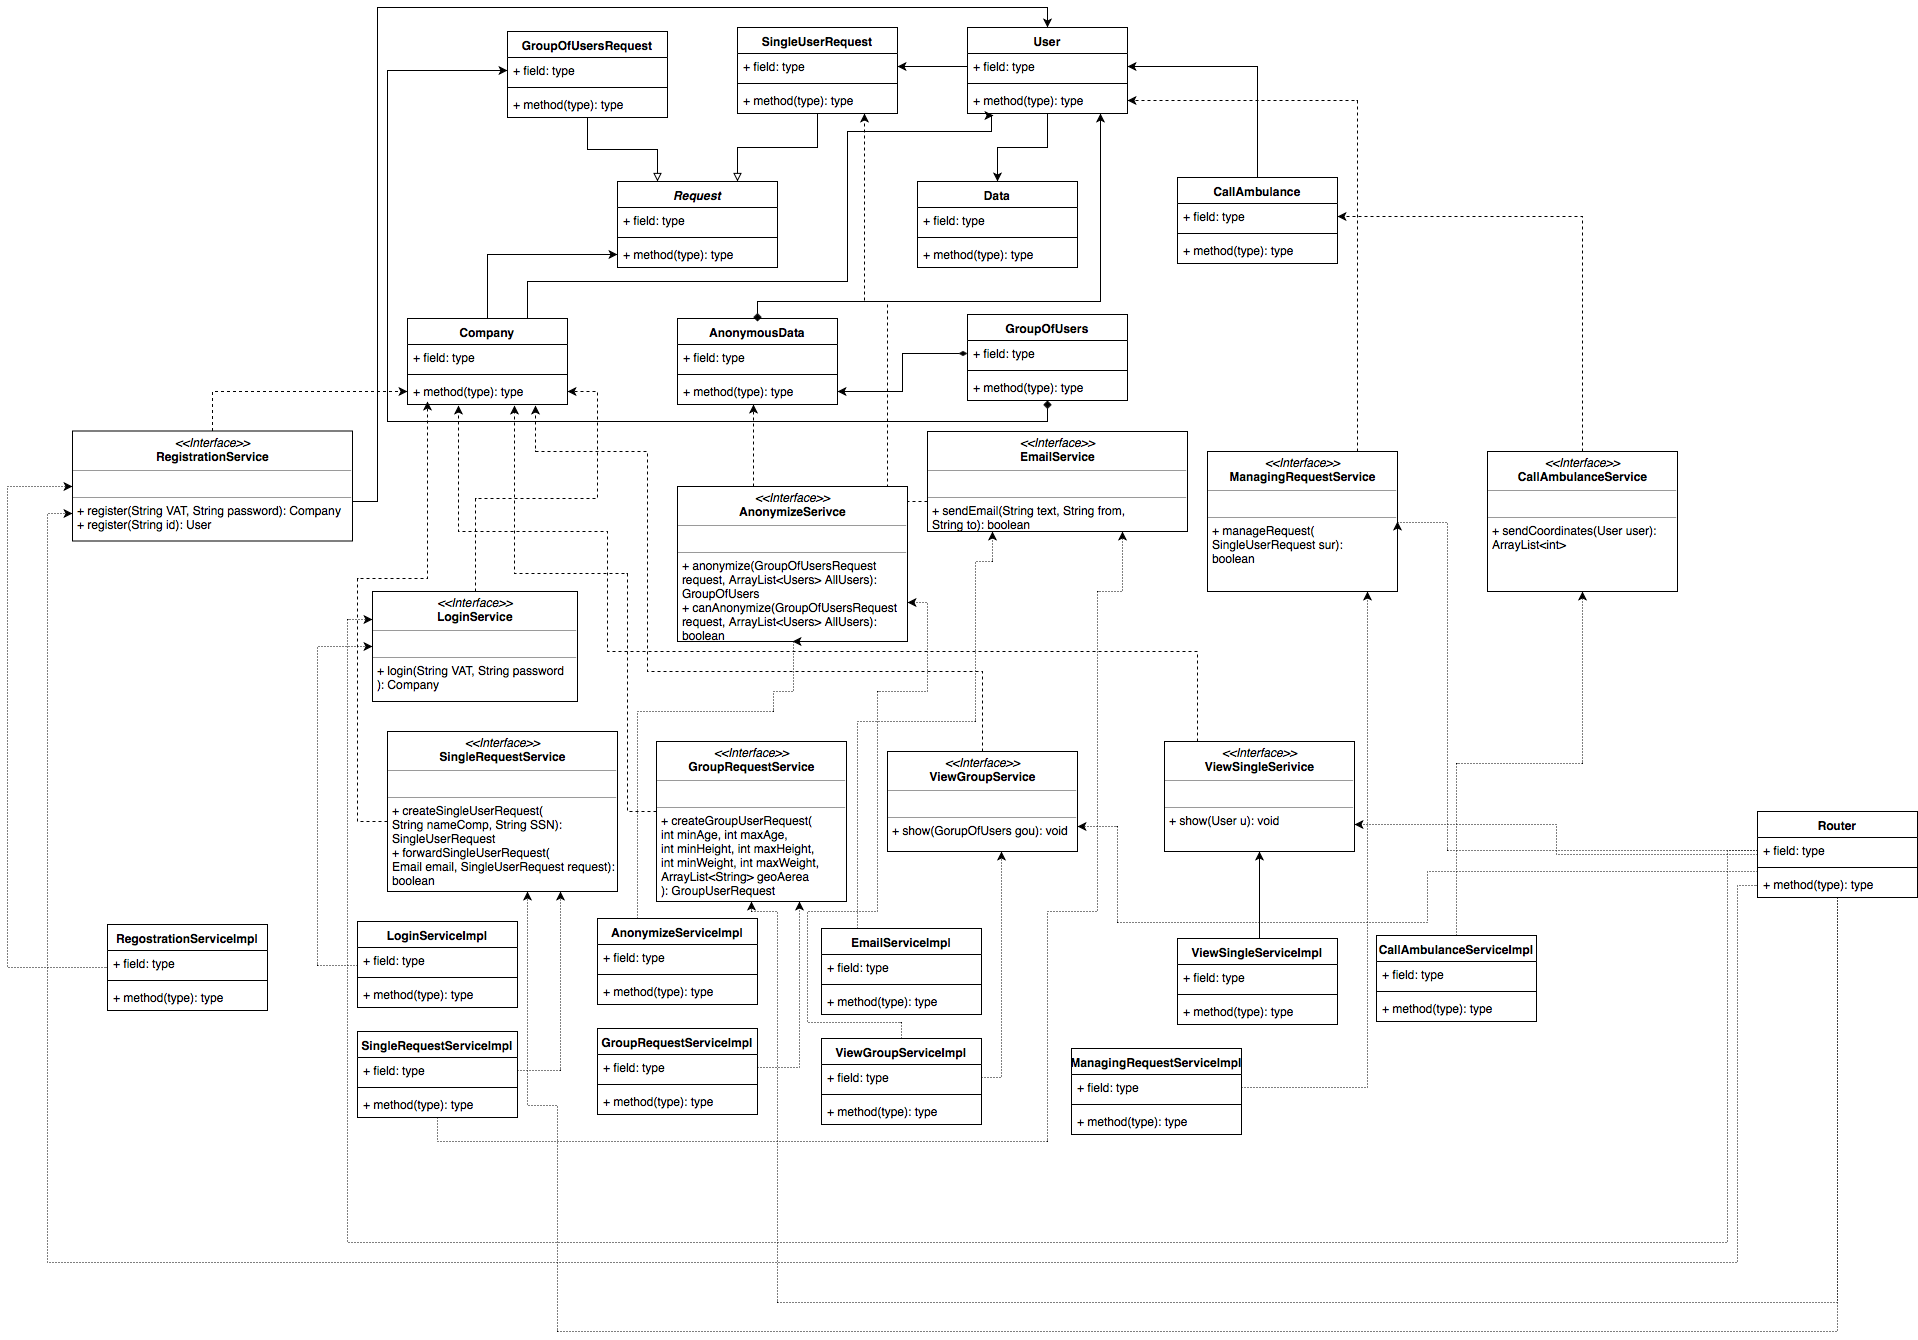
\includegraphics[width= \linewidth]{UMLbig.png}
\end{figure}
\newpage
\subsection{Deployment View}
\begin{figure}[h!]
\centering
    \textbf{}\par\medskip
	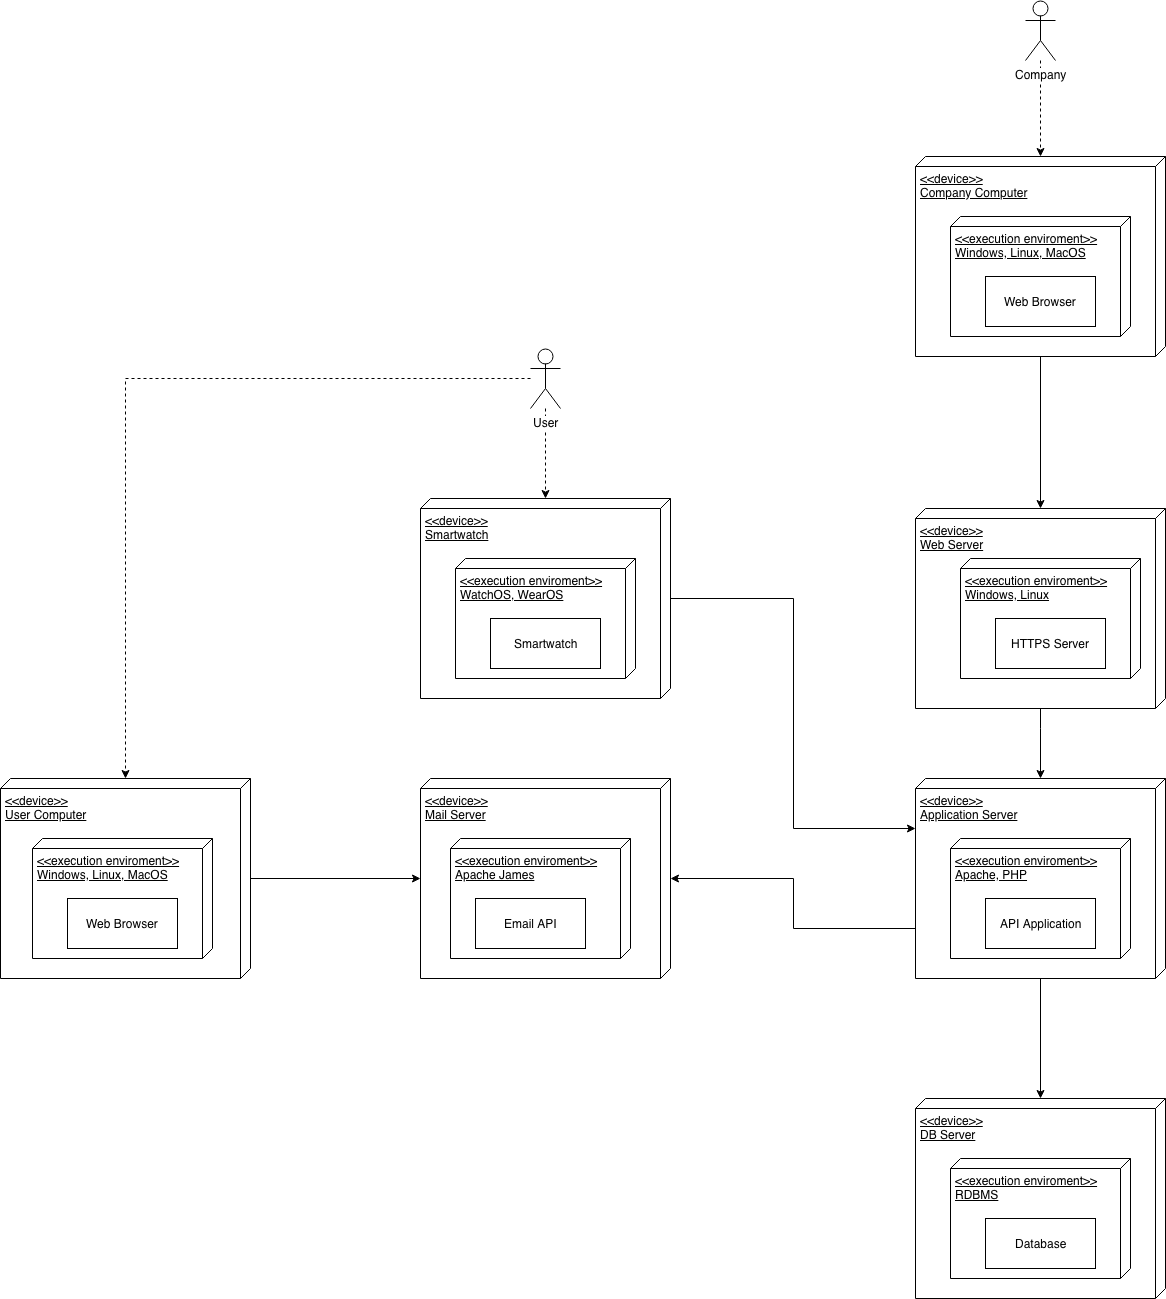
\includegraphics[width= \linewidth]{depl.png}
\end{figure}
The diagram shows the architecture of the system-to-be. Data4Help requires the deployment of software on these nodes:
\begin{itemize}
\item \textbf{smart watch}: the application runs in background in order to collect user's data and communicates them to the Application Server;
\item \textbf{User Web Browser}: the acceptance of any single user request from the user is made with his own mailbox. By clicking on the link the user is redirected on the website and the request can then be accepted or rejected;
\item \textbf{Company Web Browser}: is used to access to single user data or to anonymous data of a group of users;
\item \textbf{Application Server}: the main logic of the application will be deployed here. This server will communicate with all the other nodes - it will collect users' data and store them in the DB server, it will exploit the email server to forward companies requests and it will show to companies the users' saved data from the DB server.
\item \textbf{DB Server}: it will store all the users' data such as heart rate, current position etc., as well as all the companies requests both for groups and single users;
\item \textbf{Email Server}: provides the email service used both by the Application server to forward the companies requests and by users to accept them.
\end{itemize}
\subsection{Runtime View}
\begin{figure}[h!]
\centering
    \textbf{}\par\medskip
	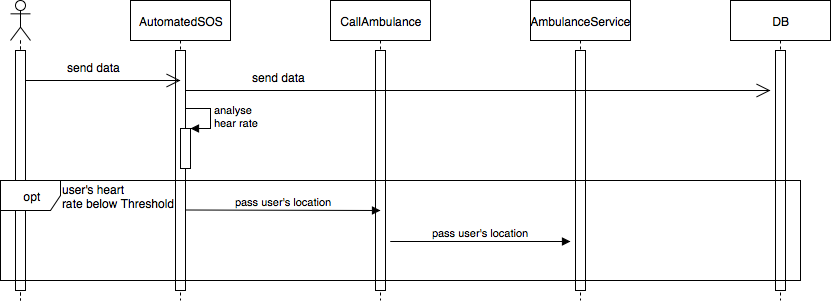
\includegraphics[width= \linewidth]{callambulance.png}
\end{figure}
In this diagram a user, registered to AutomatedSOS, sends with his smart watch his bio-medical parameters and his current location to the System-To-Be. Since the user is already registered to AutomatedSOS there is no necessity to ask for his data, but can access them directly.\newline
Every time that AutomatedSOS recevies new data it checks if they are below a threshold. If so creates an instance of a CallAmbulance class that is responsible for contacting the AmbulanceService and sending the user location.
\newpage
\begin{figure}[h!]
\centering
    \textbf{}\par\medskip
	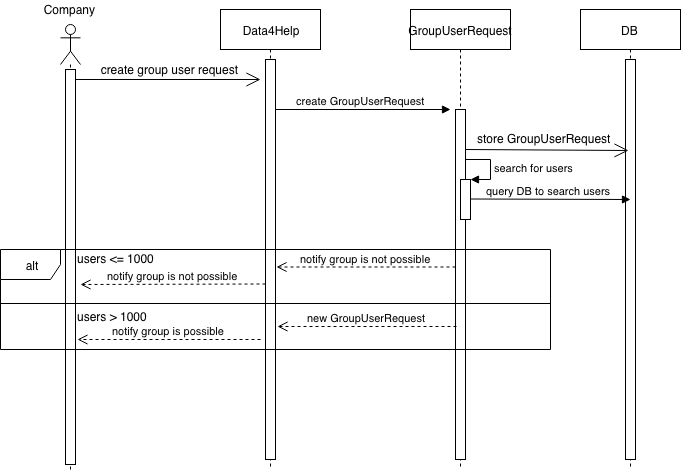
\includegraphics[width= \linewidth]{grouprequest.png}
\end{figure}
In this diagram a company creates a group user request, to identify the group they can use various filters (e.g. age, ZIP Code, etc.). The Group User Request is stored in the DB. The system searches for the users corresponding to the filters by querying the DB.\newline
The outcome depends on the number of users found: if there are more than 1000 the outcome is positive, a group is created and the company is notified; otherwise the system is notified that a group doesn't exist and also the company is notified.
\newpage
\begin{figure}[h!]
\centering
    \textbf{}\par\medskip
	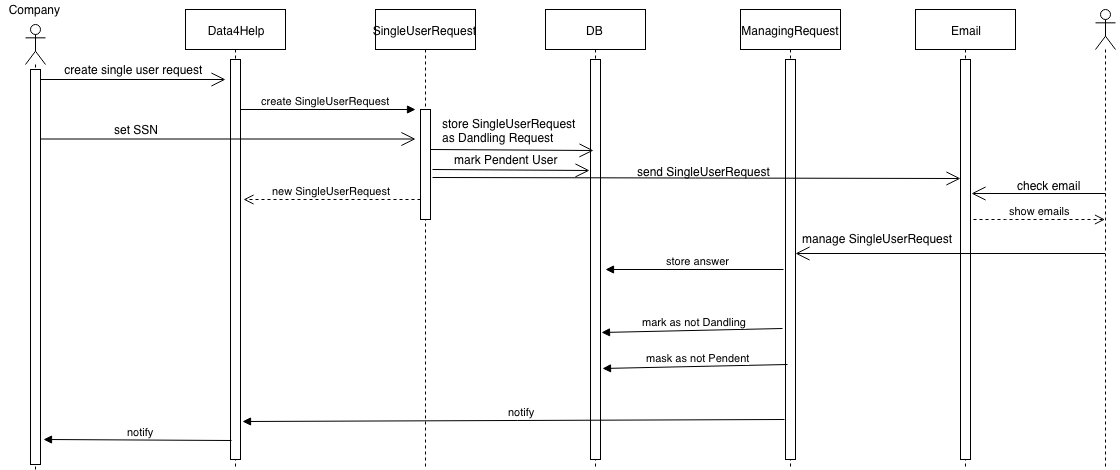
\includegraphics[width= \linewidth]{singlerequest.png}
\end{figure}
In this diagram a company creates a single user request by using a SSN.  The single user request is stored in the DB as dandling request and the user is marked as a Pendent User. The request is sent to the user by email, he can choose whether accepting it or not by clicking the corresponding link in the email. The link redirects the user into a web page that interacts with the Managing Request Service. The user's answer is stored in the DB, he is marked as not pendent anymore and the request is marked as not dandling as well. In the end the system and the company are notified of the outcome.
\newpage
\subsection{Component Interfaces}
This diagram shows the interaction between different component interfaces, this information was already present in the class diagram, but here it is shown more clearly.
\begin{figure}[h!]
\centering
    \textbf{}\par\medskip
	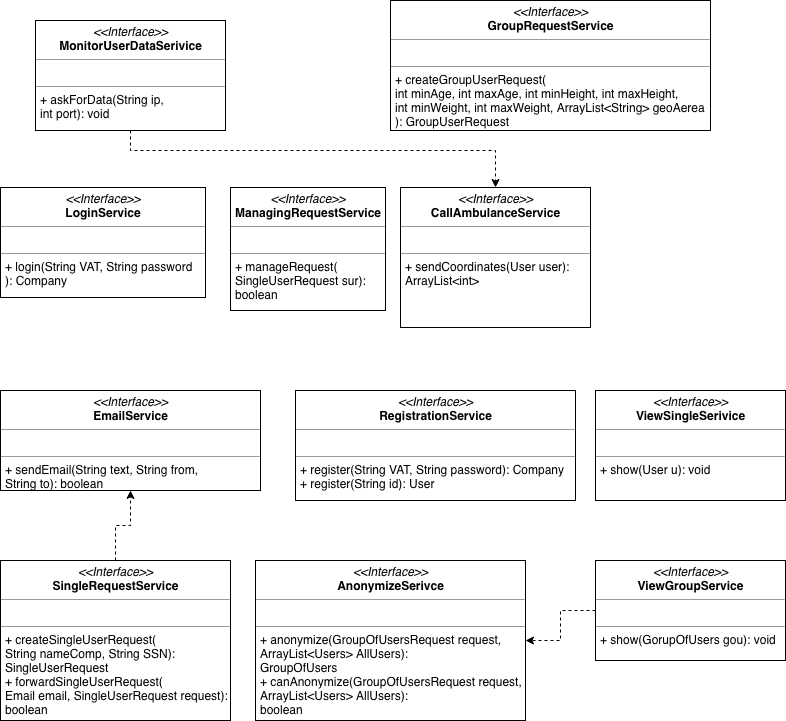
\includegraphics[width= \linewidth]{inter.png}
\end{figure}
\newpage
\subsection{Selected Architectural styles and patterns}
\subsubsection{Overall Architecture}
Our application uses a three-tiers architecture. \newline
The first tier is composed of the presentation tier and the "Tier One", respectively the first is relative to the company and the second is relative to the user.The presentation tier is the only layer that company can access by using the web browser that displays all the corresponding services; Tier One is used by the user in order to communicate his data to the App server. Both of them communicate only with the Business Logic Tier. \newline
The second tier, the Business Logic one, controls the application's functionality by performing processing on users' data and is where lies all the logic that manages with the single or group requests. \newline
The data tier, or Presistence tier, is where all the data are permanently stored.
\subsubsection{Design Pattern}
Recommended architectural pattern:
\begin{itemize}
\item Model - View - Controller (MVC): The model is the central component of the pattern. It is the application's dynamic data structure, independent of the user interface. It directly manages the data, logic and rules of the application. The view is any output representation of information. The controller, accepts input and converts it to commands for the model or view.
In addition to dividing the application into three kinds of components, the model–view–controller design defines the interactions between them.
The model is responsible for managing the data of the application. It receives user input from the controller. The view means presentation of the model in a particular format. The controller responds to the user input and performs interactions on the data model objects. The controller receives the input, optionally validates it and then passes the input to the model.
\item Client - Server: The client-server characteristic describes the relationship of cooperating programs in an application. The server component provides a service to many clients, which initiate requests for such services. The client only has to understand the response based on the well-known application protocol. Clients and servers exchange messages in a request–response messaging pattern. The client sends a request, and the server returns a response. All client-server protocols operate in the application layer. This pattern has been chosen for different reasons:
\begin{itemize}
\item It’s pratical.
\item Data synchronization: there is only one application that manage the data.
\item Having one unique server application improves the maintenability.
\item the application is independent from the number of clients connected.
\item improves the security between clients, that known only the server endpoint
but not other clients.
\end{itemize}
\end{itemize}
Recommended behavioral pattern:
\begin{itemize}
\item Observer: lets one or more objects be notified of state changes in other objects within the system. It is useful for the AutomatedSOS external service, in order to observe the data coming from the user and in case instantiate the CallAmbulance class.
\end{itemize}
\subsection{Other Design Desicions}
The users data should be sampled at regular intervals, i.e. every 5 seconds. \newline
The system uses the email external service in order to let the user accept or reject companies' requests.
\newpage
\section{User Interfaces Design}
The mock-ups for this application have already been presented in the RASD Document.
\section{Requirements Traceability}
Here is presented the mapping between the RASD goals and software components:
\begin{itemize}
	\item {[G1]} Visitor can become User after providing credentials. (Requirement \textbf{[R1]})
	\begin{itemize}
	\item RegistrationServiceImpl
	\end{itemize}
	\item {[G2]} User can accept or reject the request of access to his data formulated by companies. (Requirements \textbf{[R2] - [R3]})
	\begin{itemize}
	\item ManagingRequestServiceImpl
	\item EmailServiceImpl
	\end{itemize}
	\item {[G3]} If user's parameters are below specified thresholds, an ambulance is called within 5 seconds. (Requirement \textbf{[R4]}) 
	\begin{itemize}
	\item CallAmbulaceServiceImpl
	\item ViewSingleUserDataServiceImpl
	\end{itemize}
	\item {[G4]} Company can sign up as Company to Data4Help and AutomatedSOS. (Requirement \textbf{[R5] - [R6]})
	\begin{itemize}
	\item RegistrationServiceImpl
	\end{itemize}
	\item {[G5]} Company can be recognized providing a password and vat number. (Requirement \textbf{[R7]})
	\begin{itemize}
	\item LoginServiceImpl
	\end{itemize}
	\item {[G6]} Company can formulate a request to see anonymized data of a group of users. (Requirement \textbf{[R8]-[R9]})
	\begin{itemize}
	\item GroupRequestServiceImpl
	\end{itemize}
	\item {[G7]} Company can formulate a request to see data of a specific user providing his SSN. (Requirement \textbf{[R9]-[R10]})
	\begin{itemize}
	\item SingleUserRequestServiceImpl
	\end{itemize}
	\item {[G8]} Company can see anonymized data of a group of users. (Requirement \textbf{[R11]-R[12]-R[13]})
	\begin{itemize}
	\item ViewGroupDataServiceImpl
	\item AnonymizeGroupDataServiceImpl
	\end{itemize}
	\item {[G9]} Company can see data of a specific user providing his SSN. (Requirement \textbf{[R14]})
	\begin{itemize}
	\item ViewSingleUserDataServiceImpl
	\end{itemize}
	\item {[G10]} Company can subscribe to users' new data. (Requirement \textbf{[R15]})
	\begin{itemize}
	\item ViewSingleUserDataServiceImpl	
	\item ViewGroupDataServiceImpl
	\item AnonymizeGroupDataServiceImpl
	\end{itemize}
	\item {[G11]} Data4Help can forward companies' requests to users. (Requirement \textbf{[R9]-[R16]})
	\begin{itemize}
	\item SingleUserRequestServiceImpl
	\item EmailServiceImpl
	\end{itemize}
	\item {[G12]} A user of Data4Help becomes a user of AutomateSOS if he is older than \emph{Age} (Requirement \textbf{[R17]-R[18]-R[19]})
	\begin{itemize}
	\item RegistrationServiceImpl
	\end{itemize}
\end{itemize}
\newpage
\section{Implementation, Integration and Test Plan}
\subsection{Implementation Plan}
In the next pages a step-by-step plan of module development is presented. \\
In order to achieve a complete test coverage of all the functionalities that the system-to-be must have, we suggest to adopt a bottom-up approach. This means that once a module is build, it has to be tested individually and then it can be integrated with other already tested modules. This methodology also drives the implementation plan, that is build considering the way and the order in which tests will be run.\\ It turns out that the already presented components can be integrated following this list: 
\begin{enumerate}
\item Model 
\item MonitorUserDataServiceImpl
\item CallAmbulanceServiceImpl
\item AnonymizeGroupDataServiceImpl
\item SingleUserRequestServiceImpl, GroupUserRequestServiceImpl, ManagingRequestServiceImpl
\item ViewSingleUserDataServiceImpl, ViewGroupDataServiceImpl
\item RegistrationServiceImpl, LoginServiceImpl
\end{enumerate}
The Model is the first component to be implemented. This is done in order to build the common ground over which the system-to-be will operate. Doing the Model as first component will force programmers to develop the project having in mind what are the data structures to deal with and their semantics in the system-to-be. \\
Once the Model is done, MonitorUserDataServiceImpl must be developed. This is the component that every 30 seconds receives data from all the smartwatches and writes them in the DB. Since all the other operations that the system-to-be needs to carry out are somehow related to data, the first component to implement must be MonitorUserDataServiceImpl. \\
The next component that is suggested to implement is CallAmbulanceServiceImpl. This is the core component of AutomatedSOS. Since AutomatedSOS is basically supplied through this component, it must be developed and tested in the very initial stages of the development process. This will allow to show stakeholders a product that has at least the core functionality. \\
The third block to develop is AnonymizeGroupDataServiceImpl. It is used by the ViewGroupDataServiceImpl so it must be surely developed before this module, and it is used by the system-to-be, to ask GroupUserRequest, so it also must be developed before this component. \\
The fourth block of components that need to be developed are those related with the \emph{requests} issued by companies. Supposed to have completed the previous steps, these modules will let programmers test a product that almost has all the relevant functionalities, since the visual display of the result is not a logical function per se. \\
The development of the remaining blocks can be done in parallel since they are not related.  
\subsection{Integration and Test Plan}
\begin{figure}[h!]
\centering
    \textbf{}\par\medskip
	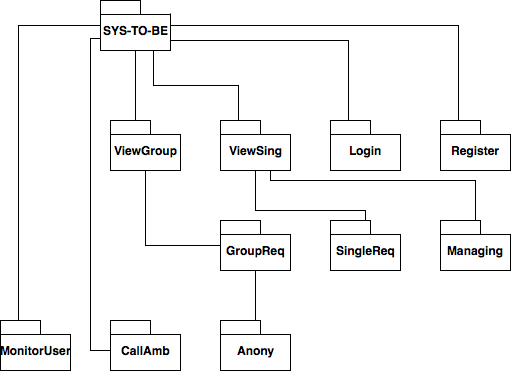
\includegraphics[width= \linewidth]{Test.png}
\end{figure}
Here is presented a representation of how the system-to-be must be integrated. \\
How was previously stated in the implementation plan, in the development of the modules programmers should be driven by the tests to be performed over the system-to-be. \\
The test plan is carried out following the bottom-up approach. \\
This methodology gives the possibility to test each functionality in isolation and to integrate it in the final system after having tested it with the modules that use it. This process is time consuming and also quite tiresome for programmers, but it forces them to test each functionality as soon as it is produced. \\
So far the Model was not mentioned, but this is just because it is not a functionality, nevertheless it is obvious that all the different modules can be tested \emph{if and only if} the Model is implemented and tested. 
\newpage
\section{Effort Spent}
\subsection{Dalle Rive Fabio}
\begin{center}
    \begin{tabular}{ | l | r |}
    \hline
    \textbf{Task Description} & \textbf{Hours} \\ \hline
    Introduction & 2\\ \hline
   	Architectural Design & 8\\ \hline
   	Diagrams & 10\\ \hline
    User Interfaces Design & 0.5\\ \hline
    Requirements Traceability & 5\\ \hline
    Implementation, Integration and Test Plan & 3\\ \hline
    \end{tabular}
\end{center}
\subsection{Di Giacomantonio Marco}
\begin{center}
    \begin{tabular}{ | l | r |}
    \hline
    \textbf{Task Description} & \textbf{Hours} \\ \hline
    Introduction & 3\\ \hline
   	Architectural Design & 7\\ \hline
   	Diagrams & 11\\ \hline
    User Interfaces Design & 0.5\\ \hline
    Requirements Traceability & 4\\ \hline
    Implementation, Integration and Test Plan & 1\\ \hline
    \end{tabular}
\end{center}
\newpage
\section{Resources}
\subsection{Used Tools}
\begin{itemize}
\item Texmaker 5.0.3
\item Adobe Photoshop
\item https://www.draw.io
\end{itemize}
\subsection{References}
\begin{itemize}
\item Specification document “Mandatory Project Assignment AY 2018-2019"
\item Software Engineering 2 Course Slides
\end{itemize}
\newpage
\end{document}


